\chapter[Analiza zmogljivosti obla"cne storitve DigitalOcean]{Analiza zmogljivosti obla"cne storitve DigitalOcean}

\pagestyle{fancy}
\fancyhf{}
\fancyhead[LE,RO]{\thepage}
\fancyhead[RE,LO]{\leftmark}

\huge "Ziga Kokelj, Tadej Hiti,\\Miha Bizjak, Matej Kristan
\normalsize
\bigskip

\section{Opis problema} \label{8_opis_problema}
\noindent Dana"snje dni se vse bolj uveljavljajo obla"cne storitve~\cite{8_servers}, saj so s stali"s"ca uporabnika najenostavnej"se za uporabo. Poleg tega imamo na voljo vse hitrej"se internetne povezave. Posledi"cno ra"cunska mo"c klientov pada in se to delo prena"sa na oddaljene stre"znike.  Na"sa naloga je implementirati prenos datoteke na obla"cno storitev, nad to datoteko na stre"zniku izvesti neke operacije ter obdelano datoteko poslati nazaj klientu. Na"sa operacija nad datoteko bo sortiranje "stevil. Na sliki \ref{8_opis_problema} je grafi"cen prikaz opisanega problema. Na"se testiranje bo obsegalo merjenje razli"cnih izvajalnih "casov na podlagi katerih bi pri"sli do podatkov o zmogljivosti sistema. Breme obla"cnega sistema bodo datoteke razli"cnih velikosti, ki bodo vsebovale naklju"cno generirana "stevila in odjemalci, ki bodo po"siljali datoteke. Obla"cna storitev bo vsebine datotek uredila po izbranem algoritmu za urejanje "stevil. Namen na"se naloge je ugotoviti zmogljivost zastonjske obla"cne storitve z vidika razli"cnih metrik.

\begin{figure}
  \centering
    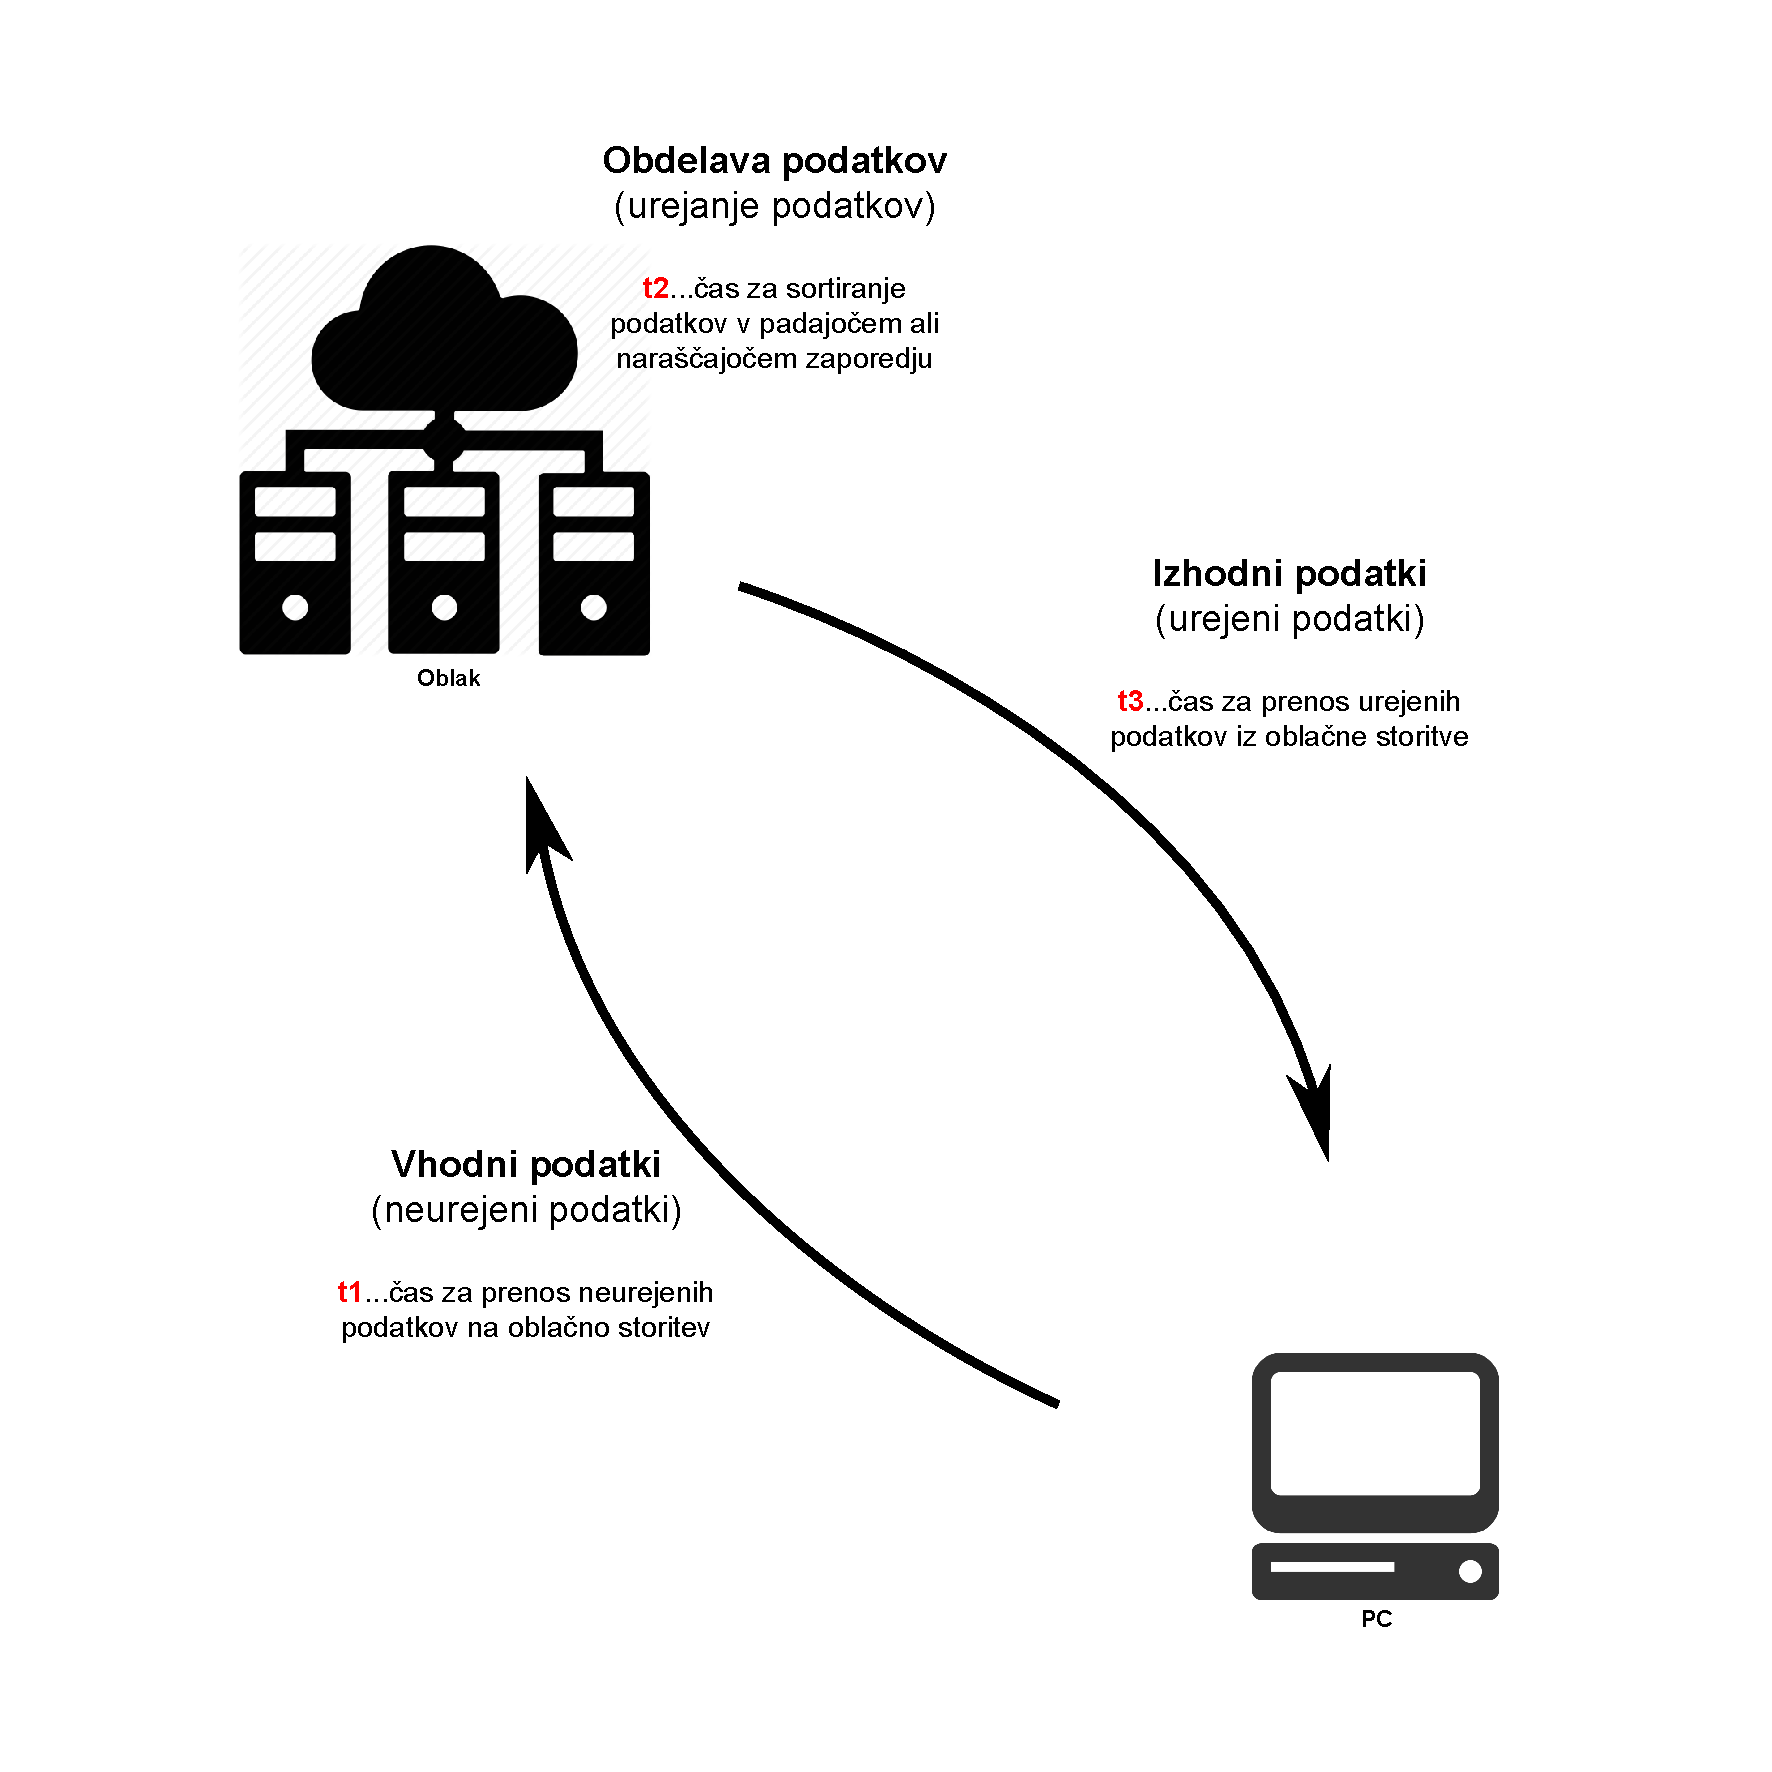
\includegraphics[width=0.74\textwidth]{8_zzrs_opis_problema.pdf}
  \caption{Shema delovanja sistema.}
  \label{8_opis_problema}
\end{figure}


\section{Izbira ponudnikov}
Zaradi brezpla"cne ponudbe preko Github Education Pack paketa za "studente smo se odlo"cili za obla"cno storitev DigitalOcean. DigtalOcean je ameri"sko podjetje, ki ponuja istoimenske obla"cne stortive. Na strani stre"znika nam ponuja izbiro razli"cnih distribucij operacijskega sistema Linux (Ubuntu, FreeBSD, Fedora, Debian, CentOS, ...).
V na"si brezpla"ci verziji imamo na voljo 512MB RAM-a, 1 procesor, 20GB prostora na SSD disku ter 1TB prenosa podatkov na mesec. V pla"cljivi razli"cici pa je na voljo vse do 64GB RAM-a, 20 procesorjev, 640GB prostora na SSD disku ter kar 9TB prenosa podatkov. Poleg velike prilagodljivosti glede zmogljivosti na"se resitve pa imamo veliko mo"znosti tudi pri izbiri fizi"cne lokacije stre"znikov. 
Izbiralo lahko med Ney Yorkom, San Franciscom, Amsterdamom, Singapurjem, Londonom, Frankfurtom, Torontom in Bangalorejem. 

\section{Izbira tehnologij}
V tem razdelku so na kratko opisane vse izbrane tehnologije, ki smo jih realizirali za na"so analizo.

\begin{figure}
  \centering
    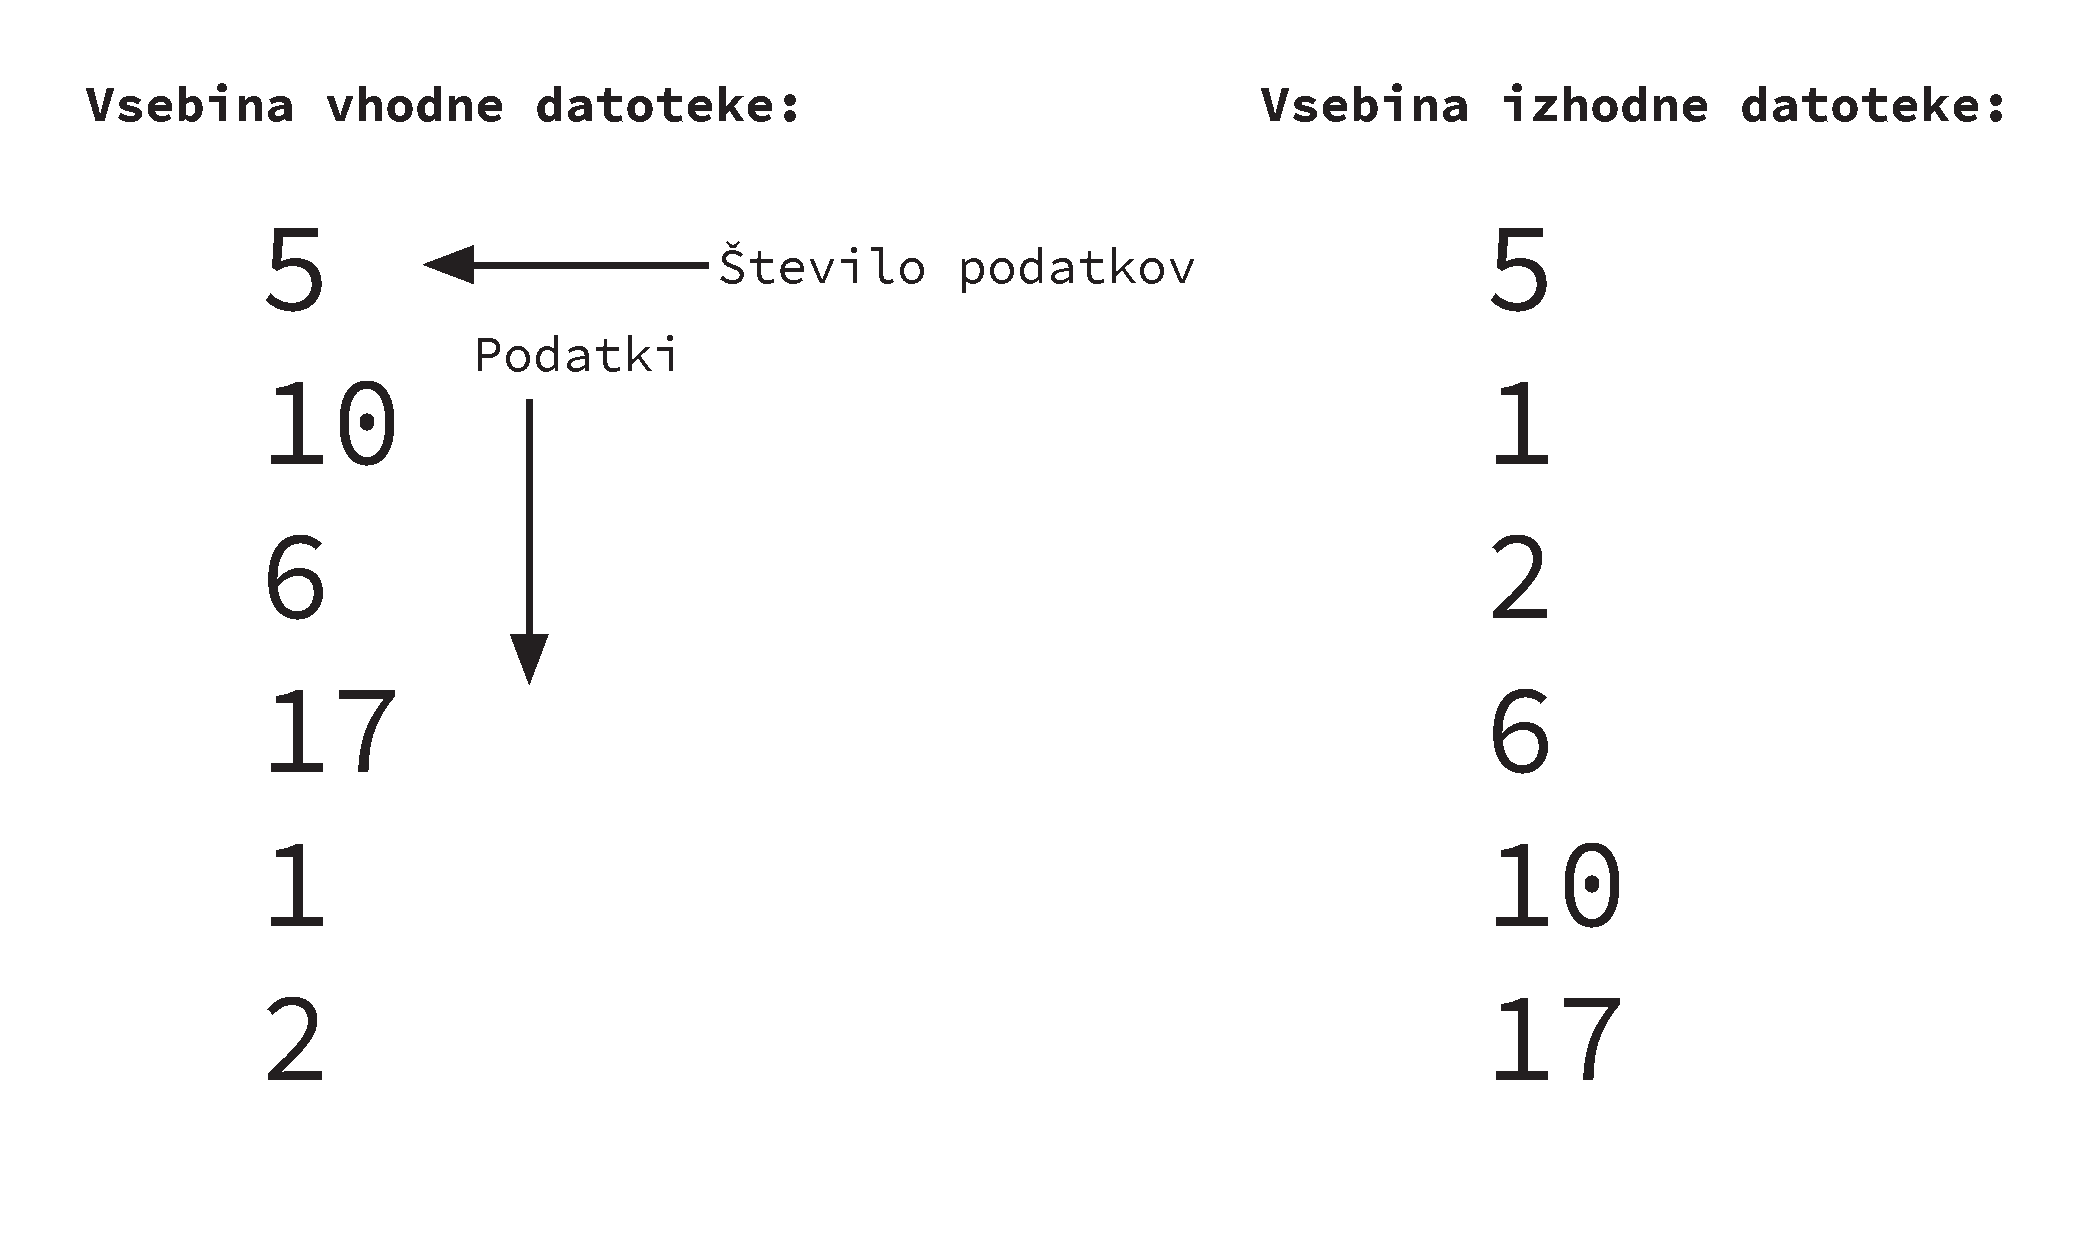
\includegraphics[width=0.75\textwidth]{ZZRS-sort_files.pdf}
  \caption{Slika prikazuje primer datoteke s katero operirata stre"znik in odjemalec.}
  \label{8_files}  
\end{figure}

\subsection{Tehnologija na strani stre"znika }
Na obla"cni stortivi DigialOcean smo implementirali stre"znik, ki je napisan v jeziku javascript z uporabo knji"znice Node.js~\cite{8_nodejs}. Stre"znik "caka na HTTP zahteve. Na 'POST /' zahtevo odgovori z html datoteko, preko katere lahko nalo"zimo datoteko, in jo z klikom na gumb po"sljemo s 'POST /nalozi' zahtevo na stre"znik. Ko stre"znik sprejme datoteko za"zene program napisan v programskem jeziku C, ki uredi podatke po vrsti v novo datoteko z algoritmom prikazanim na sliki \ref{8_sort}, z $O(n^2)$ "casovno zahtevnostjo. Program prejeto datoteko bere po vrsticah, kjer prva  vrstica vsebuje "stevilo podatkov, nasljednje vrstice pa podatke. Urejeno datoteko stre"znik po"slje, kot odgovor odjemalcu. 

\subsection{Tehnologija za avtomatizacijo odjemalcev}
Zaradi avtomatskega testiranja smo napisali skripto v programskem jeziku python~\cite{8_python}, ki omogo"ca avtomatsko po"siljanje datoteke preko URL 'POST /nalozi' zahteve na stre"znik, ter po"caka na datoteko z urejenimi podatki, kot odgovor. Seveda ob tem zabele"zimo "se "cas pred po"siljanjem zahteve in "cas po prejetju urejene datoteke, da dobimo izvajalni "cas celotne procedure. Ker je odjemalcev lahko ve"cje "stevilo, smo ta problem re"sili z nitmi, kjer vsaka nit predstavlja enega odjemalca in po"silja zahteve na stre"znik, preko istega IP naslova.

\subsection{Generiranje vhodnih podatkov}
V programskem jeziku C smo napisali generator datotek, ki ustvari datoteko željene velikosti z naklju"cnimi "srevili. Za Test1 smo generirali datoteke velikosti: 10000, 20000, 30000, 40000 in 50000 "stevil tipa integer.

\subsection{Uporabljeni algoritmi za sortiranje}
\begin{figure}
  \centering
    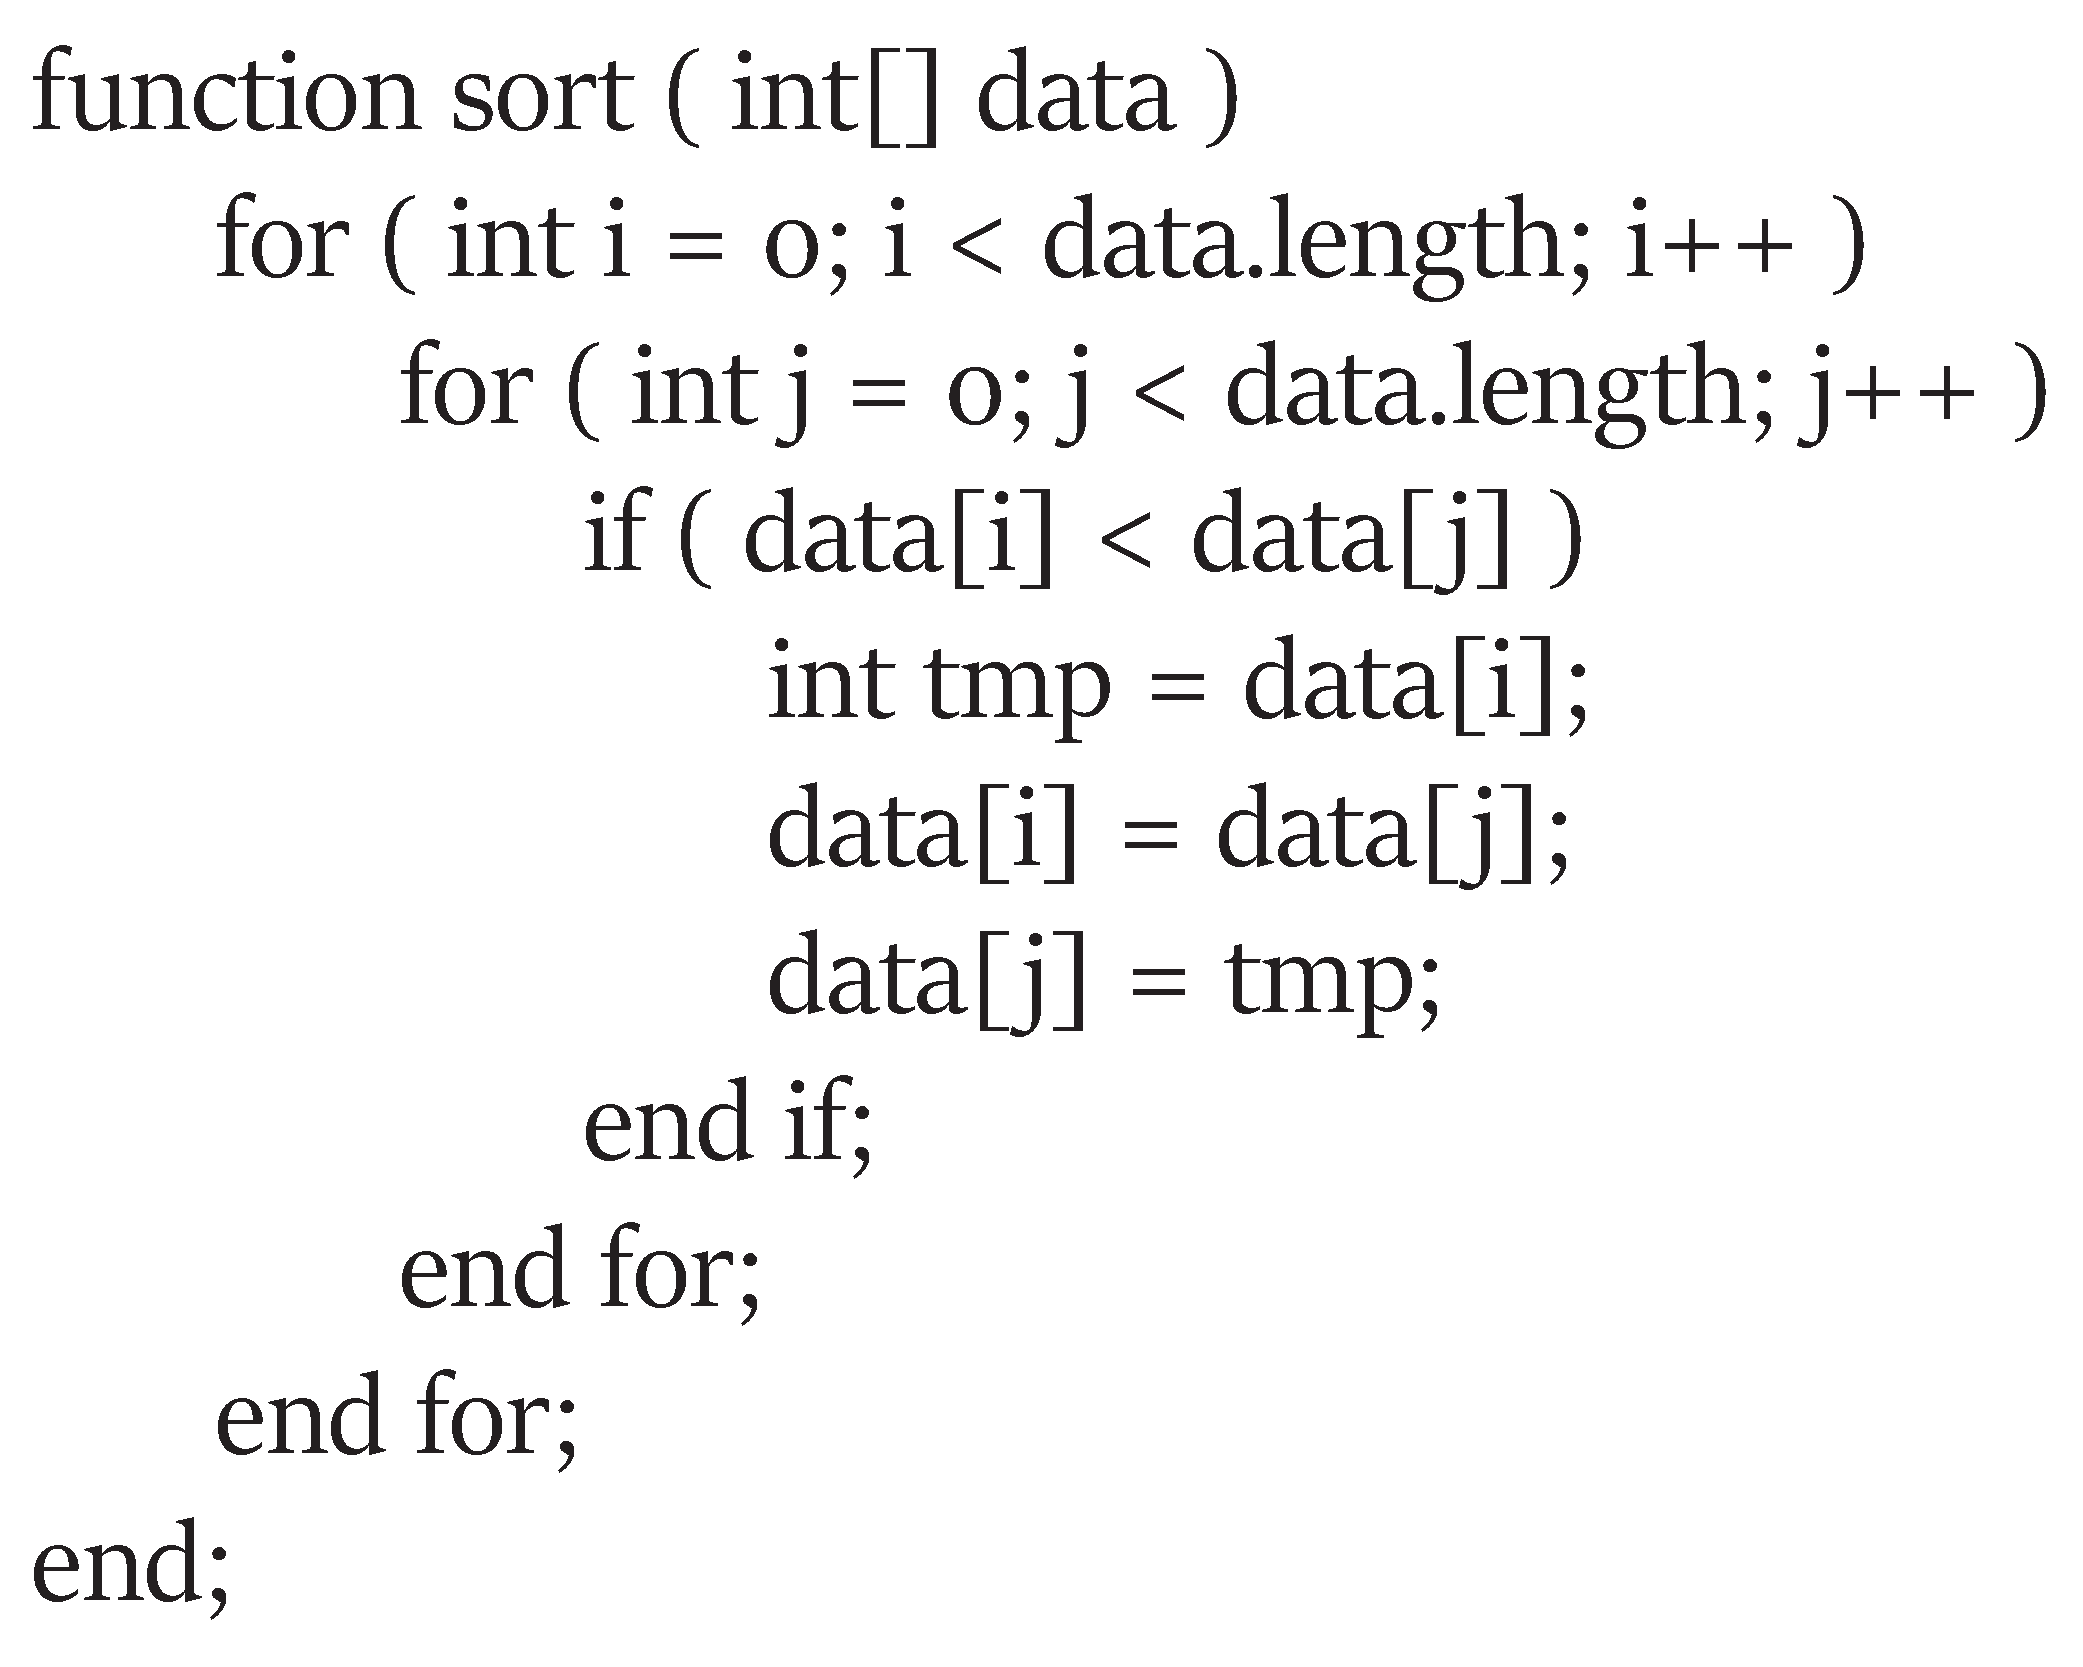
\includegraphics[width=0.65\textwidth]{ZZRS-sort_simple.pdf}
  \caption{Slika prikazuje algoritem sortiranja z $O(n^2)$ "casovno zahtevnostjo.}
  \label{8_sort}  
\end{figure}

\section{Testiranje I. }
Testiranje je bilo izvedeno med 18:00 in 22:00 v "cetrtek 18. Maja 2017 iz "studentskega naselja Ro"zna Dolina. Za dostop je bila uporabljana internetna povezava s hitrostjo prenosa 100Mbps in nalaganja 100Mbps.
Stre"znik te"ce na operacijskem sistemu Ubuntu 16.04 in ima na voljo 512MB RAM-a, 1 procesor, 20GB prostora na SSD disku in je lociran v Frankfurtu(Nem"cija). Na stre"zniku je bil izbran algoritem bubble sort \ref{8_sort}

\subsection{Nacin testiranja}
Testiranje smo izvedli s pomo"cjo generiranih datotek. Namenski program v Python-u je prakti"cno hkrati poslal datoteko na 1, 10, 20, 30 in 40 odjemalcev. Da bi zagotovili ve"cjo to"cnost podatkov smo test ponovili s po petimi datotekami v vsakem velikostnem razredu. 
Izmerili smo vse povpre"cne case ter iz njih izra"cunali povpre"cje ter standardno deviacijo, kar lahko vidite na spodnjem grafu  \ref{8_test1} . 

\subsection{Rezultati meritev}
Poleg ponujanja stre"zni"skih stortiev nam DigitalOcean nudi tudi grafi"cni prikaz porabe posameznih rezisrov(CPE, RAM, DISK, ...).
Grafe porabe resursov lahko vidite na spodnjem grafu. 

\begin{figure}
  \centering
    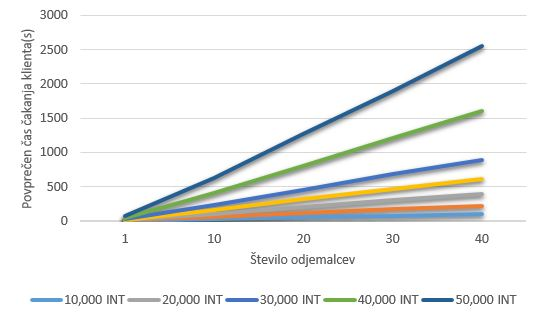
\includegraphics[width=1.0\textwidth]{test_frankfurt1.jpg}
  \caption{Graf "casa obdelave v odvisnosti od "stevila odjemalcev in velikosti datotek.}
  \label{8_graph_frankfurt1}
\end{figure}



\begin{figure}[!htbp]
  \centering
  \begin{tabular}{ | c | c | c | }
    \hline
    "Stevilo odjemalcev & Povpre"cni cas obdelave[s] & Standardna deviacija\\ \hline
    1 & 16.059     & 0 \\ \hline
    10 & 103.792 & 1.625\\ \hline
    20 & 205.444 & 4.881\\ \hline
    30 & 300.890 & 12.827\\ \hline
    40 & 393.277 & 14.598\\ \hline
  \end{tabular}
  \caption{Tabela "casov obdelav datoteke z 20 tiso"c integer "stevili.}
  \label{8_table1}
  \centering
\end{figure}



\begin{figure}
  \centering
    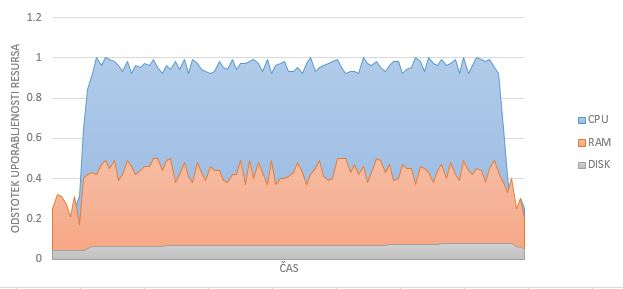
\includegraphics[width=1.0\textwidth]{resources_frankfurt1.jpg}
  \caption{Graf zasedenosti resursov med izvajanjem testov.}
  \label{8_test1_res}
\end{figure}

\subsection{Razlaga meritev}
Ob ogladu meritev opazimo, da "cas "cakanja posameznega odjemalca na datoteke v povpre"cju nara"s"ca pribli"zni linearno glede na "stevilo odjemalcev, ki hkrati po"sljejo datoteko.
Naklon grafa je mo"cno odvisen od velikosti sortiranih datotek in pri ve"cjih datotekah na ve"c odjemalcih precej naraste.
Iz grafa zasedenosti resursov lahko razberemo, da je "sibka tocka na"sega sistema procesor, saj je ta skoraj ves "cas izvajanja testov 100% obremenjen. RAM nikoli med testiranjem ne preseže 50% zasedenosti.
Najmanj obremenjena komponenta je trdi disk, saj vsako datoteko po obdelavi sproti izbri"se.

\section{Testiranje II. }
Testiranje je bilo izvedeno med 10:00 in 14:00 (po lokalnem času 1:00 do 5:00)  v ponedeljek 22. Maja 2017 iz "studentskega naselja Ro"zna Dolina. Za dostop je bila uporabljana internetna povezava s hitrostjo prenosa 100Mbps in nalaganja 100Mbps.
Stre"znik te"ce na operacijskem sistemu Ubuntu 16.04 in ima na voljo 512MB RAM-a, 1 procesor, 20GB prostora na SSD disku in je lociran v San Franciscu(Vzhodna obala ZDA). Na stre"zniku je bil izbran algoritem bubble sort \ref{8_sort}


\subsection{Nacin testiranja}
Testiranje smo izvedli s pomo"cjo generiranih datotek. Namenski program v Python-u je prakti"cno hkrati poslal datoteko na 1, 10, 20, 30 in 40 odjemalcev. Da bi zagotovili ve"cjo to"cnost podatkov smo test ponovili s po petimi datotekami v vsakem velikostnem razredu. 
Izmerili smo vse povpre"cne case ter iz njih izra"cunali povpre"cje ter standardno deviacijo, kar lahko vidite na spodnjem grafu  \ref{8_test1} . 

\subsection{Rezultati meritev}
Poleg dobljenih "casov meritev smo pridobili tudi podatke o zasedenosti resursov na streni stre"znika. Zasedenost resursov je zelo podobna zasedenosti pri prvem testiranju. 


\begin{figure}
  \centering
    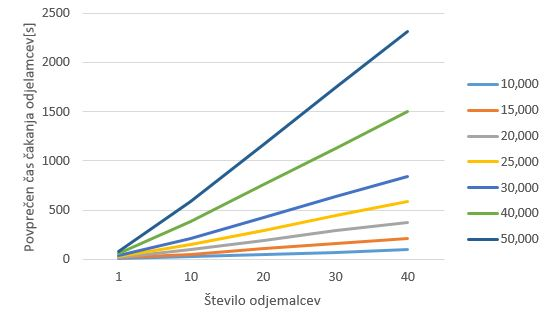
\includegraphics[width=1.0\textwidth]{test_sanfrancisco1.jpg}
  \caption{Graf "casa obdelave v odvisnosti od "stevila odjemalcev in velikosti datotek.}
  \label{8_graph_sanfrancisco1}
\end{figure}



\begin{figure}[!htbp]
  \centering
  \begin{tabular}{ | c | c | c | }
    \hline
    "Stevilo odjemalcev & Povpre"cni cas obdelave[s] & Standardna deviacija\\ \hline
    1 & 22.659     & 0 \\ \hline
    10 & 100.001 & 6.552\\ \hline
    20 & 190.552 & 10.279\\ \hline
    30 & 288.468 & 8.757\\ \hline
    40 & 377.072 & 19.697\\ \hline
  \end{tabular}
  \caption{Tabela "casov obdelav datoteke z 20 tiso"c integer "stevili.}
  \label{8_table_sanfrancisco1}
  \centering
\end{figure}


\subsection{Razlaga meritev}
Rezultati meritev so zelo podobni rezultatom meritev na stre"zniko v Frankfurtu..
TODO: Dopi"si razlago!


\section{Testiranje III. }
Testiranje je bilo izvedeno med 00:30 in 2:30 v torek 23. Maja 2017 iz "studentskega naselja Ro"zna Dolina. Za dostop je bila uporabljana internetna povezava s hitrostjo prenosa 100Mbps in nalaganja 100Mbps.
Stre"znik te"ce na operacijskem sistemu Ubuntu 16.04 in ima na voljo 2GB RAM-a, 2 procesorja, 20GB prostora na SSD disku in je lociran v Frankfurtu(Nem"cija). Na stre"zniku je bil izbran algoritem bubble sort \ref{8_sort}

\subsection{Nacin testiranja}
Testiranje smo izvedli s pomo"cjo generiranih datotek. Namenski program v Python-u je prakti"cno hkrati poslal datoteko na 1, 10, 20, 30 in 40 odjemalcev. Da bi zagotovili ve"cjo to"cnost podatkov smo test ponovili s po petimi datotekami v vsakem velikostnem razredu. 
Izmerili smo vse povpre"cne case ter iz njih izra"cunali povpre"cje ter standardno deviacijo, kar lahko vidite na spodnjem grafu  \ref{8_test1} . 

\subsection{Rezultati meritev}
Poleg dobljenih "casov meritev smo pridobili tudi podatke o zasedenosti resursov na streni stre"znika. 
TODO: zasedenost resursov


\begin{figure}
  \centering
    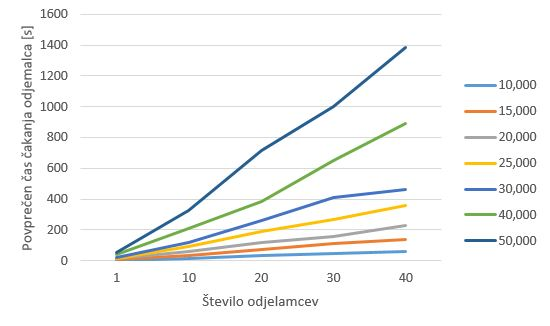
\includegraphics[width=1.0\textwidth]{test_frankfurt2.jpg}
  \caption{Graf "casa obdelave v odvisnosti od "stevila odjemalcev in velikosti datotek.}
  \label{8_graph_frankfurt2}
\end{figure}



\begin{figure}[!htbp]
  \centering
  \begin{tabular}{ | c | c | c | }
    \hline
    "Stevilo odjemalcev & Povpre"cni cas obdelave[s] & Standardna deviacija\\ \hline
    1 & 22.659     & 0 \\ \hline
    10 & 100.001 & 6.552\\ \hline
    20 & 190.552 & 10.279\\ \hline
    30 & 288.468 & 8.757\\ \hline
    40 & 377.072 & 19.697\\ \hline
  \end{tabular}
  \caption{Tabela "casov obdelav datoteke z 20 tiso"c integer "stevili.}
  \label{8_table_sanfrancisco1}
  \centering
\end{figure}




\subsection{Razlaga meritev}
Rezultati meritev so zelo podobni rezultatom meritev na stre"zniko v Frankfurtu..
TODO: Dopi"si razlago!

\section{Primerjava "casov na razli"cnih stre"znikih z datotekami velikosti 10,000 INT}

\subsection{Graf}
\begin{figure}
  \centering
    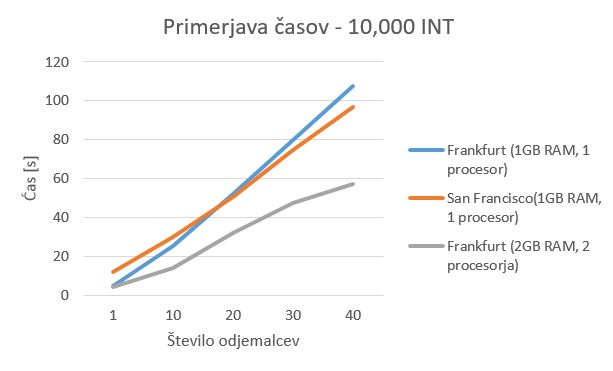
\includegraphics[width=1.0\textwidth]{comparison_10000.jpg}
  \caption{Primerjava povpre"cnih casov na treh razli"cnih stre"znikih.}
  \label{8_graph_comparison_10000}
\end{figure}

\subsection{Razlaga}
Pri majhnem "stevilu odjemalcev opazimo razliko v temu, da imata oba stre"znika v Frankfurtu ni"zje "case, kar lahko pojastnimo z bli"zjo fizi"cno razdaljo med nami(klientom) in stre"znikom. 
Pri vi"sjem "stevilu odjemalcev je hitrej"si enako zmogljiv stre"znik v San Franciscu, kot v Frankfurtu. To je najbr"z posledica "casa testiranja, saj je bil stre"znik v Frankfurtu testiran zvečer, v San Franciscu pa sredi no"ci, ko je obremenjenost praviloma manj"sa.
Iz grafa lahko tudi lepo vidimo, da je "cas cakanja klientov precej manj"si pri pri zmogljivej"sem stre"zniku. Razlika se pri ve"canju stevila odjemalcev "se pove"cuje.

\section{Primerjava "casov na razli"cnih stre"znikih z datotekami velikosti 20,000 INT}

\subsection{Graf}
\begin{figure}
  \centering
    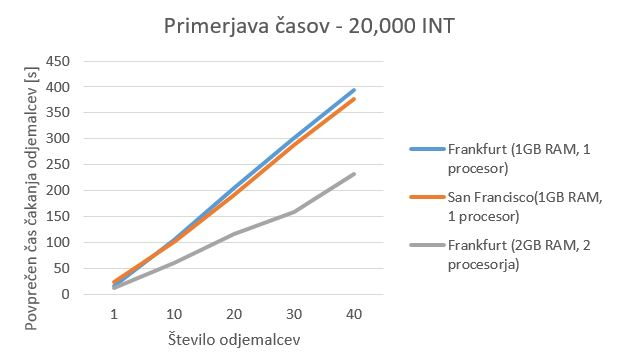
\includegraphics[width=1.0\textwidth]{comparison_20000.jpg}
  \caption{Graf "casa obdelave v odvisnosti od "stevila odjemalcev in velikosti datotek.}
  \label{8_graph_comparison_20000}
\end{figure}

\subsection{Razlaga}
Iz grafa lahko razberemo, da je fizi"cna oddaljenost stre"znika velikega pomena le, dokler sistem ni popolnoma obremenjen. To se zgodi pri le enem klientu in tu stre"znika v Frankfurtu hitreje opravita svoje delo, kot tisti v San Franciscu.
Pri vi"sjih obremenitvah pa bolj do izraza bolj pride obremenjenost stre"znika. "Se vedno je povpre"cni "cas "cakanja odvisen od zmogljivosti stre"znika. 


\section{Primerjava "casov na razli"cnih stre"znikih z datotekami velikosti 50,000 INT}

\subsection{Graf}
\begin{figure}
  \centering
    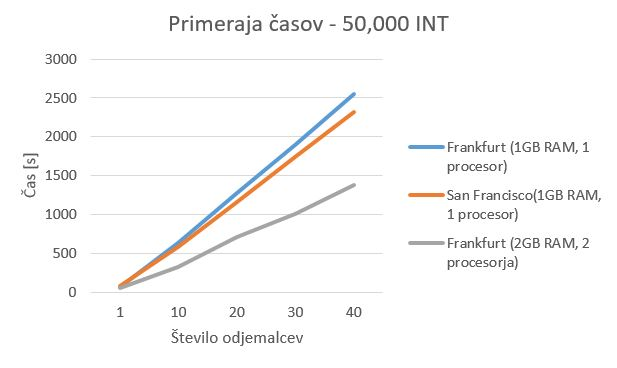
\includegraphics[width=1.0\textwidth]{comparison_50000.jpg}
  \caption{Graf "casa obdelave v odvisnosti od "stevila odjemalcev in velikosti datotek.}
  \label{8_graph_comparison_50000}
\end{figure}

\subsection{Razlaga}
TODO: razlaga	






